\chapter{Herramienta Web. \emph{Front-End}}
\label{frontend}
Nuestra aplicación Web está dividida en \emph{back-end} y \emph{front-end}. En el capítulo anterior se describió el \emph{back-end}. El propósito de
este capítulo es describir el \emph{front-end}, que es el encargado de la capa de presentación.
\par
El \emph{front-end} se implementa en JavaScript\cite{JavaScript}. Este es un lenguaje de programación soportado por la mayoría de navegadores, que
permite dotar de funcionalidad extra a las páginas Web. Actualmente el uso de este lenguaje está tan extendido y avanzado que permite crear
aplicaciones enteras para navegadores Web. Existen múltiples frameworks escritos en JavaScript que facilitan la creación de aplicaciones Web. En este
trabajo utilizamos dos: Sencha ExtJs\cite{ExtJs} y HighStock\cite{HighStock}.
\par
Sencha ExtJs es un framework orientado a la creación de aplicaciones Web interactivas. Se trata de un framework de propósito general que ofrece
abstracciones para gestionar nuestros datos, arquitectura MVC, componentes gráficos de control y otros. 
\par
HighStock es un framework con un propósito específico, que es la creación de gráficos. Podemos elegir entre diferentes tipos de gráficos, que pueden
ser: lineas, barras, áreas, \emph{candlestick} y otros. Los gráficos generados son altamente interactivos lo que permite ocultar series, navegar,
realizar zoom y mucho más.
\par
Empezaremos este capítulo aclarando los aspectos técnicos relacionados con estos dos frameworks. Explicaremos como usarlos, que funcionalidad nos
proporcionan, consideraciones que debemos tener en cuenta.
\par
Como podemos ver en la figura \ref{frontend} nuestro \emph{front-end} está basado en el patrón de diseño
\emph{modelo-vista-controlador}\cite{MVCWiki}. En la segunda parte de este capítulo hablaremos más a fondo sobre la división impuesta por este patrón
de diseño.
\begin{figure}[h]
	\centering
	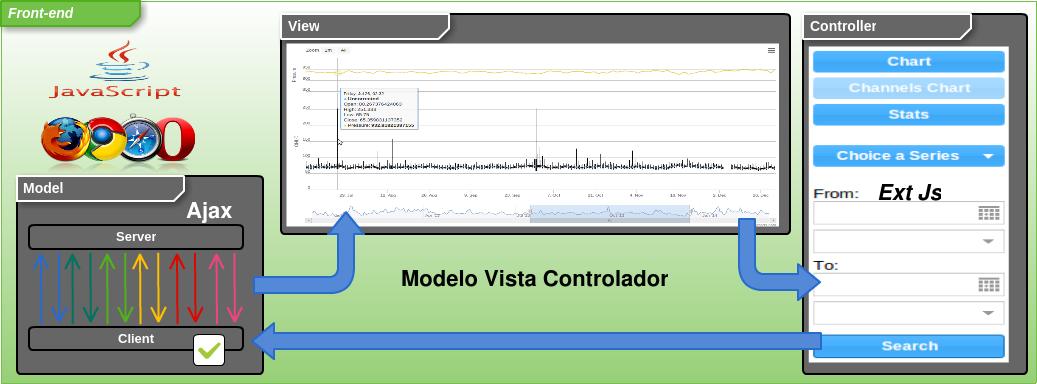
\includegraphics[keepaspectratio, width=1\textwidth]{./img/frontend.png}
	\caption{\emph{Front-end}. Patrón MVC.}   
	\label{fig:frontend}
\end{figure}
\par
En nuestra aplicación también hacemos una división funcional, diferenciamos entre tres módulos que son \texttt{Spike}, \texttt{SpikeRevised} y
\texttt{ChannelStats}. En las secciones finales de este capítulo hablaremos sobre estos módulos. 

\section{Sencha ExtJs}
	El propósito de esta sección es explicar alguno de los aspectos básicos del framework. Empezaremos explicando como crear una aplicación básica
	con ExtJs. En la mayoría de los casos existe un único documento HTML\cite{HTML} que contiene toda la aplicación. En él tenemos que cargar dos
	\emph{scripts} de la siguiente forma.
    		\begin{center} \texttt{<script type="text/javascript" src=\textquotedbl extjs/ext-all-debug.js\textquotedbl ></script>}  \end{center}
    		\begin{center} \texttt{<script type="text/javascript" src=\textquotedbl app.js\textquotedbl ></script>}  \end{center}
	El primer \emph{script} contiene el framework que queremos utilizar. Es conveniente destacar que esta es una versión concebida para el proceso
	de desarrollo. Para la versión final es conveniente usar el \texttt{ext-all.js}, que es una versión comprimida del mismo \emph{script}.
 	\par
	El segundo \emph{script} es el que contiene la lógica de nuestra aplicación. A continuación podemos ver un ejemplo del código mínimo que este
	\emph{script} debe contener. El código presentado se explicará a fondo.
	\begin{lstlisting}[style=myJs]
Ext.application({
   name: 'HelloExt',
   launch: function() {
      Ext.create('Ext.container.Viewport', {
         layout: 'fit',
            items: [{
               title: 'Hello Ext',
               html : 'Hello! Welcome to Ext JS.'}] 
      }); 
   } 
});
	\end{lstlisting}
	\par
	En la primera línea hacemos uso del singleton \texttt{Ext}. Este es un objeto que encapsula todas las clases y métodos proporcionados por el
	framework. La función utilizada \texttt{Ext.application} carga e inicializa una instancia de la clase \texttt{Ext.app.Application}. Esta clase
	representa una aplicación ExtJs \emph{single-page}. La llamada a esta función crea la variable global \texttt{MyApp}, que debe contener todas las
	clases e instancias de nuestra aplicación.
 	\par
	En la segunda línea declaramos el nombre de nuestra aplicación. Seguidamente definimos la función \texttt{launch}. Esta función es ejecuta
	cuando se lanza la aplicación. La primera función invocada es \texttt{Ext.create} que crea una instancia de la clase proporcionada, en este
	caso \texttt{Ext.container.Viewport}. \texttt{Viewport} es un \emph{contenedor} que representa el área de aplicación y puede haber tan sólo
	uno por aplicación. 
 	\par
	La interfaz de usuario en una aplicación ExtJs se compone de \emph{componentes}. Un \emph{contenedor} es un \emph{componente} especial que
	contiene otros \emph{componentes}. En la figura \ref{fig:comps} podemos ver un ejemplo que ilustra esta jerarquía.
	\begin{figure}[h]
		\centering
		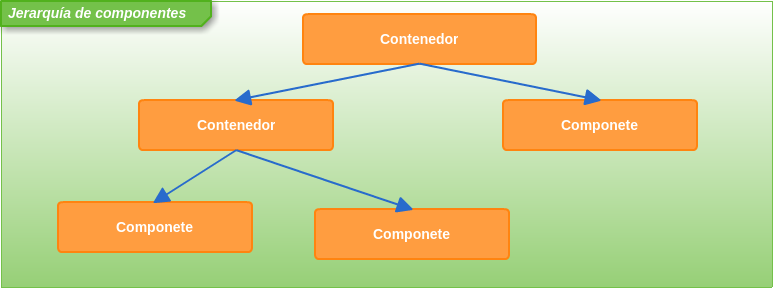
\includegraphics[keepaspectratio, width=1\textwidth]{./img/comps.png}
		\caption{Sencha ExtJs. Jerarquía de componentes.}   
		\label{fig:comps}
	\end{figure}
 	\par
	El \texttt{Viewport} es el \emph{contenedor} que gestiona el área de representación del navegador Web. Los \emph{compenentes} de un
	\emph{contenedor} se especifican en el campo \texttt{items} que es una lista. En el ejemplo presentado tan sólo tenemos un \emph{componente},
	pero pueden añadirse más.
 	\par
	Fijándonos en el código de ejemplo podemos ver que antes de definir el campo \texttt{items} definimos el campo \texttt{layout}. El
	\texttt{layout} especifica la forma en la que se posicionan y ajustan los \emph{componentes} hijos dentro del padre. En este caso el
	\texttt{layout} especificado es \texttt{\cc fit\cc}, donde un único hijo ocupa todo el espacio del padre.
	\subsection{Component Manager}
		ExtJs ofrece el singleton \texttt{Ext.ComponentManager} que provee un registro con todos los componentes. Este facilita la referencia
		a elementos desde cualquier punto del código. El propósito de esta sección es explicar como hacer uso de esta facilidad.
		\par
		Empezaremos especificando un requisito que  los componentes deben cumplir, estos deben definir el atributo \texttt{itemId}. Este
		atributo es el identificador del componente. El ámbito que tiene este identificador es local al contenedor que contiene el componente.
		Esto hace que los identificadores no tengan que ser únicos para toda la aplicación. 
		\par
		Es el singleton \texttt{Ext.ComponentQuery} el que permite realizar búsquedas de componentes en función del \texttt{itemId}.
		Concretamente es \texttt{Ext.ComponentQuery.query()} el método que permite realizar las búsquedas. Este método acepta dos parámetros.
		El primer parámetro, \texttt{selector}, es un String y especifica el \texttt{itemId} que queremos buscar. El segundo parámetro,
		\texttt{root} es opcional y especifica el contenedor dentro de cual queremos hacer la búsqueda. Si el segundo parámetro se omite la
		búsqueda se realizará entre todos los componentes. La función devuelve un array con todos los componentes que reúnen las condiciones,
		pudiendo ser un array vacío. Eventualmente podemos hacer búsquedas más complejas, que nos permiten buscar por tipo, atributos y mucho
		más. En este trabajo tan sólo hemos utilizado consultas simples.
		\par
		La clase \texttt{Ext.container.Container} implementa las funciones \texttt{down()} y \texttt{query()}. Estas dos realizan una llamada
		a \texttt{Ext.ComponentQuery.query()} teniéndose a si mismo como parámetro \texttt{root}. Esto les permite hacer una búsqueda entre
		sus hijos.
		\par
		También existe el método \texttt{up()} implementado por \texttt{Ext.Component}. Este permite hacer una búsqueda similar a las
		anteriormente descritas. En este caso se navega hacia arriba en la jerarquía de componentes y se busca por componentes que reúnan los
		criterios. Esta función puede ser invocada sin ningún parámetro, caso en el que devuelve el padre inmediato del componente.
		\par
		Es conveniente citar el parámetro \texttt{id} y la función \texttt{Ext.getCmp()}. Estos dos ofrecen una funcionalidad parecida a la
		anteriormente explicada, pero no deben ser usados con ese propósito. Estan considerados como obsoletos y pueden dar lugar a
		colisiones. 
	\subsection{Layouts}
		El propósito de esta sección es explicar los \texttt{layouts} utilizados en este trabajo. Tal y como explicamos anteriormente, el
		\texttt{layout} especifica la forma en la que se posicionan y ajustan los componetes hijos dentro del padre. Tan sólo explicaremos la
		funcionalidad de estos sin centrarnos en el uso que les hemos dado, este será explicado en las secciones venideras cuando proceda. En
		la figura \ref{fig:layouts} podemos ver una representación de los \texttt{layouts} que describiremos a continuación.
		\begin{description}[style=unboxed,leftmargin=0cm,labelwidth=1cm]
			\item[\texttt{Absolute}] Los \emph{componentes} hijo son posicionados mediante el uso de coordenadas \texttt{X,Y}. Las
			  dimensiones de estos también se definen de forma estática mediante el uso de dos atributos, \texttt{height} and
			  \texttt{width}. La posición y tamaño de los componentes se puede cambiar mediante el uso de las funciones
			  \texttt{setPosition()} y \texttt{setSize()}.
			\item[\texttt{Accordion}] Este layout se asemeja a un acordeón. Los \emph{componentes} hijo pueden ser expandidos y
			  colapsados, teniendo tan sólo uno expandido a la vez. Los \emph{componentes} son ordenados en vertical ocupando todo el
			  espacio disponible. Las funciones \texttt{expand} y \texttt{collapse} permiten expandir y colapsar los paneles.
			  También están presentes multitud de manejadores de eventos que podemos sobrescribir. En nuestro caso hacemos uso del
			  \texttt{beforeExpand} que se dispara antes de expandir un \emph{componente}. 
			\item[\texttt{Border}] Este layout permite tener hasta cinco \emph{componentes} dispuestos de la manera que podemos ver en la
			  figura \ref{fig:layouts}. Los componentes hijos deben especificar el atributo \texttt{region} que determina la posición que
			  tendrán. El atributo puede tomar los siguientes valores: \texttt{[north, east, south, west, center]}. No es necesario que
			  estén presentes los cinco hijos, podemos omitir los que no sean necesarios.
			\item[\texttt{Card}] Este layout maneja multiples \emph{componentes} hijo. Los hijos ocupan todo el espacio disponible, por lo
			  que se solapan entre ellos. Esto hace que solamente uno sea visible a la vez. El layout asemeja una baraja de cartas donde
			  solamente una carta puede estar en la parte superior. La función que permite hacer visible un hijo es \texttt{setActiveItem()}.
			  Esta función acepta el \emph{componente}, el \texttt{itemId} o el índice de este.
			\item[\texttt{Fit}] Este es un layout muy simple, que tan sólo acepta un hijo, y este ocupa todo el espacio que el padre ofrece.
			  El \emph{componente} hijo se expande automáticamente para ajustarse al tamaño del padre.
			\item[\texttt{HBox y VBox}] Estos son dos layouts diferentes, pero muy parecidos. \texttt{HBox} organiza sus elementos hijos
			  de forma horizontal a lo largo del \emph{componente} padre. \texttt{VBox} hace lo mismo, pero la organización es de forma
			  vertical. Los componentes hijos pueden especificar el atributo \texttt{flex}, que determina como será repartido el
			  espacio disponible entre los diferentes hijos. Para ilustrar el funcionamiento del \texttt{flex} expondremos un ejemplo.
			  Teniendo dos \emph{componentes} hijo con \texttt{1} y \texttt{2} de \texttt{flex} respectivamente, el primero ocupará 1/3 y
			  el segundo 2/3 del espacio total.
		\end{description}
		\begin{figure}[h]
			\centering
			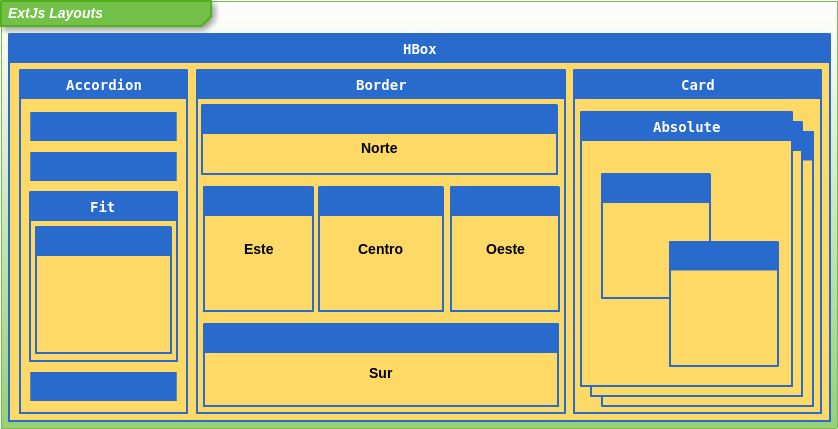
\includegraphics[keepaspectratio, width=1\textwidth]{./img/layouts.png}
			\caption{Sencha ExtJs. Layouts.}   
			\label{fig:layouts}
		\end{figure}

	\subsection{Lazy instantiation}
		La inicialización perezosa es una técnica que consiste en retrasar la creación de recursos hasta el momento en el que sea necesario su
		uso. Como hemos visto en la sección dedicada a los layouts en muchos casos los componentes no son visibles. Tener que crear todos los
		componentes al inicializar la aplicación no es muy eficiente, dado que tan sólo unos pocos son visibles. Crear tan sólo los
		componentes visibles según se vayan necesitando supone un incremento en el rendimiento. En páginas pequeñas con pocos componentes el
		aumento no es apreciable, sin embargo en páginas que manejan multitud de componentes el incremento puede ser drástico. 
		\par
		Para implementar esta inicialización perezosa ExtJs se basa en la jerarquía de componentes previamente explicada. Cuando un componente
		es creado también se crean todos los componentes hijos que deben ser visibles en ese momento. Tal y como explicamos los componentes
		hijos se definen en el campo \texttt{items}. A continuación podemos ver un pequeño ejemplo. 
		\begin{lstlisting}[style=myJs]
items:[
   Ext.create('Ext.form.field.Text',{
      fieldLabel:'Foo'}),
   Ext.create('Ext.form.field.Text', {
      fieldLabel: 'Bar'})]
		\end{lstlisting}
		\par
		El ejemplo presentado anteriormente no habilita la inicialización perezosa. Para este propósito tenemos que evitar el uso de la
		función \texttt{Ext.create()}. Tenemos que especificar los componentes hijos como objetos de configuración. A continuación se presenta
		un ejemplo.
		\begin{lstlisting}[style=myJs]
items: [{
   xtype: 'textfield',
   fieldLabel: 'Foo'},
{
   xtype: 'textfield',
   fieldLabel: 'Bar'}]
		\end{lstlisting}
		\par
		La diferencia que podemos apreciar entre los dos ejemplos es el atributo \texttt{xtype}. Este especifica la clase que tendrá el
		componente.  Como podemos ver no se especifica el nombre completo de la clase. \texttt{xtype} acepta una serie de atajos para
		referenciar a las clases. En nuestro caso la clase \texttt{Ext.form.field.Text} es referenciada por el \texttt{xtype:\cc
		textfield\cc}.
		\par
		La lista completa de \texttt{xtypes} aceptados se puede consultar en la documentación de ExtJs\cite{ExtJsDoc}. Eventualmente podemos
		extender esta lista declarando nuestros propios \texttt{xtypes}. Esto se hace especificando el campo \texttt{xtype} a la hora de
		definir nuestra clase. A continuación presentamos un pequeño ejemplo.
		\begin{lstlisting}[style=myJs]
Ext.define('MyApp.PressMeButton', {
   extend: 'Ext.button.Button',
   xtype: 'pressmebutton',
   text: 'Press Me'});
		\end{lstlisting}

	\subsection{Events}
		Las clases y componentes de ExtJs disparan multitud de eventos a lo largo de su ciclo de vida. Los eventos se disparan cuando algo
		interesante le ocurre a nuestro componente. Un ejemplo es el evento \texttt{afterrender} que se dispara después de mostrar en pantalla
		el componente.
		\par
		Los eventos son muy interesantes porque podemos definir funciones, \texttt{listeners}, que se ejecutan cuando se producen dichos
		eventos. A continuación presentamos un ejemplo en el que podemos ver cómo manejar el evento \texttt{click}, que se dispara al hacer
		\emph{click} sobre un componente. 
		\begin{lstlisting}[style=myJs]
Ext.create('Ext.Button',{
   text: 'Click Me',
   renderTo: Ext.getBody(),
   listeners:{
      click: function(){
         Ext.Msg.alert('I was clicked!');}
   }
});
		\end{lstlisting}
		\par
		ExtJs también permite configurar eventos propios. Estos se declaran como si fuesen eventos normales. La peculiaridad está en que somos
		nosotros los que debemos dispararlos haciendo uso de la función \texttt{fireEvent}. Esta acepta como parámetros el evento que queremos
		disparar y todos los parámetros que la función encargada de este necesite. A continuación podemos ver un pequeño ejemplo de como
		declarar y disparar un evento propio, que tiene como nombre \texttt{myEvent}.
		\begin{lstlisting}[style=myJs]
var button = Ext.create('Ext.Button',{
   text: 'Custom Event',
   renderTo: Ext.getBody(),
   listeners:{
      myEvent: function(number){
         Ext.Msg.alert('Custom event fired, number: '+number);}
   }
});
button.fireEvent('myEvent', 42);
		\end{lstlisting}
	\subsection{Componentes}  %Muy mal. %Si sobra contenido esta sección tiene que ser eliminada.
		ExtJs ofrece multitud de componentes, que son subclases del \texttt{Ext.Component}, cada uno con un propósito diferente. El objetivo
		de esta sección es describir los componentes usados en este trabajo. Nos centraremos en los aspectos técnicos sin especificar el uso
		concreto que les hemos dado. Este será explicado en secciones futuras cuando proceda. 
		\begin{description}[style=unboxed,leftmargin=0cm]
			\item[\texttt{Ext.button.Button xtype:button}] Este componente permite crear un botón. El propósito de un botón es ofrecer un
			  medio fácil al usuario para interactuar con la aplicación. Los botones que ExtJs ofrece son altamente configurables, tanto
			  funcionalmente como estéticamente. Podemos tener botones normales, botones \emph{toggle}, botones que despliegan menús y
			  mucho más. Para dar funcionalidad a estos botones tenemos que escuchar los eventos que estos disparan. Los eventos más
			  comunes son \texttt{click}, \texttt{toggle}, \texttt{mouseover} y \texttt{mouseout}.
			\item[\texttt{Ext.form.field.Date xtype:datefield}] Este componente proporciona un campo de entrada de fecha. Es posible
			  especificar el formato deseado en el que introducir la fecha, y si este formato no es respetado el campo es subrayado en
			  color rojo indicando al usuario la inconsistencia. Eventualmente este campo puede desplegar un selector de fechas que
			  facilita el proceso de introducir la fecha deseada. Al igual que los demás componentes este dispara multitud de eventos que
			  podemos manejar.
			\item[\texttt{Ext.form.field.Time xtype:timefield}] Este componente es muy similar al anteriormente descrito, y proporciona
			  un campo de entrada de tiempo. También acepta una configuración del formato deseado y advierte  al usuario cuando este no es
			  respetado. El componente puede desplegar un selector de tiempo que facilita la tarea de introducir el valor deseado.
			\item[\texttt{Ext.form.Label xtype:label}] Este componente permite generar una etiqueta de texto. Este componente es muy
			  similar al tag HTML <label>. Este componente permite configurar múltiples aspectos y manejar múltiples eventos.
			\item[\texttt{Ext.panel.Panel xtype:panel}] Este componente es una parte fundamental en la creación de aplicaciones con ExtJs.
			  Esta pensado para ser utilizado como un contenedor, contener otros componentes. Este componente es altamente configurable
			  pero el aspecto más importante es el \texttt{layout} que determina como se posicionan los componentes hijos. 
			\item[\texttt{Ext.tab.Panel xtype:tabpanel}] Este componente es una extensión del componente anterior. Este ofrece múltiples
			  pestañas en la que organizar los componentes hijos.  Esto permite incluir una cantidad mayor de contenido en el mismo
			  espacio. La barra de pestañas que el componente ofrece es altamente configurable. 
			\item[\texttt{Ext.grid.Panel xtype:gridpanel}] Este componente es un contenedor capaz de presentar una tabla. Las tablas son
			  altamente interactivas, estas permiten al usuario ordenar los datos, hacer búsquedas, eliminar datos, añadir datos y mucho
			  más.
		\end{description}
	\subsection{History stack}
		La aplicación Web que estamos desarrollando es una aplicación \emph{single-page}. Este modelo rompe con el patrón tradicional de
		navegación por el historial usando los botones \emph{Forward/Back}. Esto presenta un problema de usabilidad cuando el usuario utiliza
		el botón de navegación hacia atrás, ya que lo esperado es volver al estado anterior de la aplicacióin. Sin embargo se carga la
		página anterior del historial y nuestra aplicación \emph{single-page} es descartada.
		\par
		La solución que la mayoría de aplicaciones \emph{single-page} han adoptado se basa en el \emph{Fragment Identifier}  o \emph{hash},
		nombre que recibe porque va precedido del símbolo \textbf{\#}. El \emph{hash} es una parte opcional de la URL que históricamente se
		utilizaba para navegar por documentos largos. Un cambio en el \emph{hash} hace que se muestren diferentes partes del documento.
		\par
		Actualmente el \emph{hash} es usado por aplicaciones \emph{single-page} para manipular la pila de historial. El hash es cambiado
		acuerdo al estado de la aplicación. Esto hace que los cambios en la aplicación sean registrados en la pila de historial.
		\par
		Al pulsar el botón de navegación hacia atrás el \emph{hash} de la URL cambia a su estado anterior. Nuestra aplicación debe ser capaz
		de detectar los cambios en el \emph{hash} y actuar acuerdo a estos. De esta manera podemos preservar la funcionalidad de los botones
		de navegación \emph{Forward/Back}. 
		\par
		Para implementar la funcionalidad anteriormente descrita ExtJs ofrece el singleton \texttt{Ext.util.History}. Para inicializar este
		módulo tenemos que invocar la función \texttt{Ext.History.init()}. Una vez inicializado este módulo podemos hacer cambios en el
		\emph{hash} invocando la función \texttt{Ext.History.add()}. Esta función acepta como parámetro el valor del \emph{hash}. 
		\par
		Para detectar y actual acorde a los cambios del \emph{hash} tenemos que inicializar un \texttt{listener}. El evento que vamos a
		capturar es \texttt{change}. A continuación podemos ver un pequeño código de como inicializar el \texttt{listener}.
		\begin{lstlisting}[style=myJs]
Ext.History.on('change', function(hash){
   switch(hash){
      case: 'Foo':
         //Actuar acuerdo al hash Foo
         break;
      case: 'Bar'
         //Actuar acuerdo al hash Bar
         break;
   };
});
		\end{lstlisting}
		\par
		El propósito de esta sección ha sido explicar el problema que surge con el historial de navegación y como prevenirlo haciendo uso del
		\texttt{Ext.History}. Del uso concreto que hemos hecho de este módulo hablaremos en secciones futuras de este capítulo.

\section{HighStock}
	El propósito de esta sección es explicar alguno de los aspectos básicos del Framework. Actualmente existen dos frameworks desarrollados por la
	misma organización, HighCharts y HighStock. Los dos framework son muy parecidos y es conveniente explicar las diferencias que existen entre
	estos. El primero tiene un propósito más general, la variedad de gráficos que permite crear es mucho más extensa. El segundo tiene un
	propósito más específico, este está enfocado a la representación gráfica de valores que evolucionan respecto al tiempo. Este enfoque es muy
	adecuado para nuestro caso. A continuación presentaremos el código mínimo necesario para crear un gráfico con HighStock. Basándose en ese
	código explicaremos los aspectos técnicos del software.
	\begin{lstlisting}[style=myJs]
myChart = new Highcharts.StockChart({
   chart: {
      renderTo: container}, //HTML element reference
   series: [{
      name: 'My First Series',
      data: myData // predefined JavaScript array
   }]
});
	\end{lstlisting}
	\par
	Como podemos ver para crear un gráfico invocamos la función \texttt{StockChart()}. Esta función acepta como parámetro un objeto que
	define la configuración del gráfico. El formato de este objeto puede verse en la documentación del framework\cite{HighStockDoc}. En nuestro
	caso tan sólo especificaremos dos atributos, la mayoría de los atributos tiene un valor por defecto por lo que no es necesario especificarlos
	explícitamente. 
	\par
	El primer atributo que especificamos es \texttt{chart}. Este atributo es un objeto que a su vez especifica  aspectos básicos del gráfico. El
	atributo que especificamos es \texttt{renderTo}, el elemento HTLM en el que nuestro gráfico será presentado.
	\par
	El segundo atributo que especificamos es \texttt{series}. Este es un array de objetos que especifican las series de nuestro gráfico. En este
	ejemplo tenemos tan sólo un objeto, por lo que nuestro gráfico tendrá tan sólo una serie.  Definiendo el atributo \texttt{name} le damos un
	nombre a nuestra serie y especificando el atributo \texttt{data} le damos datos a nuestra serie. El atributo \texttt{data} tiene que ser un
	array que contenga los datos, este array puede tener múltiples formatos que no explicaremos dado que están muy bien explicado en la
	documentación proporcionada\cite{HighStockDoc}.
	\par
	En este punto volveremos al \texttt{renderTo} a fin de explicar la integración entre HighStock y Sencha ExtJs. En secciones anteriores
	explicamos que la interfaz de usuario de una aplicación ExtJs se constituye de componentes. Estos componentes son abstracciones con
	funcionalidades muy extendidas pero en el fondo son un elemento HTML. Este elemento será asignado al atributo \texttt{renderTo} a fin de
	mostrar un gráfico HighStock en un componente de una Aplicación ExtJs. El elemento HTML de un componente es accesible de la siguiente forma.
    		\begin{center} \texttt{Ext.Component.getEl().dom}  \end{center}
	\subsection{Agrupación de datos y \emph{Candlestick}} 
		\begin{wrapfigure}{R}{0.42\textwidth}
			\centering
	        	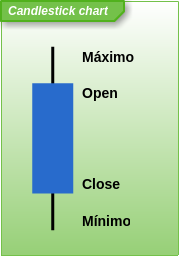
\includegraphics[keepaspectratio, width=0.40\textwidth]{./img/candlestick.png}
			\caption{Gráfico Candlestick.}
			\label{fig:candlestick}
		\end{wrapfigure}
		El objetivo de esta sección es explicar el gráfico \emph{Candlestick} o gráfico de velas. Hemos utilizado este gráfico para dar
		solución a un problema que explicaremos a continuación. Seguidamente explicaremos como interpretar este gráfico.
		\par
		El problema radica en la gran cantidad de datos que tienen que ser representados en nuestro gráfico. El sistema de adquisición genera
		una entrada de datos cada minuto, 1440 datos al día o 43200 datos al mes. Estas cantidades de datos son excesivas comparadas con las
		resoluciones de pantalla actuales. Consideremos una pantalla estándar con 1280 pixeles de ancho, es imposible representar 43200 datos.
		\par
		Para dar solución a este problema hemos recurrido a agrupar los datos. El fin es crear un número de grupos que no exceda el ancho de
		pixeles de nuestra pantalla. Para cada grupo tenemos que calcular un valor representativo. Una técnica común es calcular el valor
		medio de los grupos.  Esto tiene el inconveniente de aplanar los Spikes, algo que queremos resaltar.
		\par
		Para evitar aplanar los Spike para cada grupo calcularemos valores más representativos que la media. En concreto calcularemos cuatro
		valores, máximo, mínimo, \emph{open} y \emph{close}. El \emph{open} y \emph{close} son la media más la desviación típica y la media
		menos la desviación típica respectivamente.
		\par
		El agrupamiento de datos y cálculo de estos cuatro valores para cada grupo está implementado en el \emph{back-end}. Los servicios RPC
		que nos permiten acceder a estos datos son \texttt{nmdbOriginalGroup} y \texttt{nmdbRevisedGroup}. Estos servicios fueron explicados
		en el capítulo dedicado al \emph{back-end}, en este punto tan sólo nos interesa destacar el argumento \texttt{points} que estos dos
		servicios aceptan. Este argumento especifica el número de grupos en los que serán agrupados los datos, este será proporcional al
		número de pixeles que tenemos disponibles para representar nuestro gráfico. 
		\par
		En análisis técnico bursátil los valores \emph{open} y \emph{close} tienen su significado propio, en este trabajo representan la media
		más la desviación típica y la media menos la desviación típica respectivamente. Como podemos ver en la figura \ref{fig:candlestick} el
		\emph{open} y \emph{close} son utilizados para construir el cuerpo de las velas. Este representa los datos que se encuentran dentro de
		la desviación típica. La línea que cruza el cuerpo de la vela representa el valor máximo y mínimo para cada grupo.
		\par
		Las velas con cuerpos alargados indican grupos en los que la desviación típica es muy grande, por contrario velas con cuerpos
		contraídos indican grupos con una desviación típica pequeña. Los dos extremos, datos que fluctúan mucho o datos que no fluctúan,
		pueden ser indicativo de un mal funcionamiento. Los valores máximo o mínimo que se alejan mucho del cuerpo de la vela nos indican la
		presencia de un Spike en dicho grupo. 	
	\subsection{Ampliando HighStock}
		HighStock es construido de forma modular para facilitar la ampliación por parte de los usuarios. En este trabajo hemos ampliado el
		framework con dos funcionalidades adicionales. El propósito de esta sección es describir estas dos funcionalidades, pero primero
		explicaremos el proceso para ampliar el framework.
		\par
		La primera consideración que tenemos que tener es el ámbito o \emph{scope}, nombre que utilizaremos a lo largo de este trabajo.
		Debemos tener cuidado de no contaminar el \emph{scope} global con variables. Para este propósito debemos utilizar una función
		\emph{self-invoking}. En JavaScript esta es una función que se ejecuta inmediatamente y crea su propio \emph{scope}, de esta manera
		evitamos contaminar el \emph{scope} global. A continuación presentamos un ejemplo de como declarar una de estas funciones.
		\begin{lstlisting}[style=myJs]
(function (H) {
   var localVar,	// Variable local
   Series = H.Series;
   doSomething();
}(Highcharts));
		\end{lstlisting}
		\par
		El framework ofrece la función \texttt{wrap} que permite añadir código en una función existente. Podemos añadir dicho código antes o
		después del código inicial de la función. La función acepta tres argumentos, el objeto padre como primer argumento, el nombre de la
		función como segundo argumento y la función de sustitución como tercer argumento. La función original es pasada como el primer
		argumento de la función de sustitución. Es conveniente fijarnos en el ejemplo de código a continuación presentado para entender mejor
		el uso de la función \texttt{wrap}.
		\begin{lstlisting}[style=myJs]
H.wrap(H.Series.prototype, 'drawGraph', function (proceed) {
// Antes de la función original.
console.log("We are about to draw the graph: ", this.graph);
// Invocar la función original usando todos los argumentos menos el primero.
proceed.apply(this, Array.prototype.slice.call(arguments, 1));
// Después de la función original.
console.log("We just finished drawing the graph: ", this.graph);
});
		\end{lstlisting}
		\par  
		A continuación explicaremos las dos ampliaciones que hemos realizado sobre el framework, la primera permite realizar zoom Out y la
		segunda permite resaltar las series de un gráfico para poder inspeccionarlas mejor.
		\subsubsection{Zoom Out}
			Tal y como explicamos los gráficos creados con el framework son altamente interactivos. Entre las diferentes funcionalidades
			están las que permiten navegar por el conjunto de datos. Con navegar nos referimos a mostrar diferentes fragmentos de los
			datos. Un ejemplo de estas funcionalidades es el zoom In, que permite ampliar una sección de datos. Haciendo \emph{click} y
			arrastrando podemos seleccionar un intervalo para realizar el zoom In. Poder hacer zoom In es muy útil para inspeccionar los
			datos, el problema es que el framework no ofrece la posibilidad de realizar un zoom Out.
			\par
			En este trabajo hemos extendido el framework para incorporar dicha funcionalidad. Para este propósito hemos modificado el zoom
			In, usamos la dirección de arrastre para diferenciar entre zoom In y zoom Out. Un arrastre de izquierda a derecha realiza un
			zoom In, mientras que un arrastre de derecha a izquierda realizar un zoom Out. 
			\par
			Para poder registrar la dirección de arrastre hemos hecho uso de dos eventos, \texttt{mousedown} y \texttt{mouseup}. En cada
			evento registramos la posición de este y usamos la diferencia entre las posiciones para determinar la dirección de arrastre. A
			continuación presentamos el código. Es la variable \texttt{selectDirection} la que indica la dirección de arrastre.
			\begin{lstlisting}[style=myJs]
H.addEvent(container, 'mousedown', function (e) {
   selectFrom = chart.pointer.normalize(e).chartX;
});

H.addEvent(container, 'mouseup', function (e) {
   selectTo = chart.pointer.normalize(e).chartX;
   selectDirection = selectTo - selectFrom;													            
});
			\end{lstlisting}
			\par
			El evento que se dispara al realizar una selección es \texttt{selection}, por lo que tenemos que registrar un manejador para
			el evento. La primera acción es comprobar el estado del \emph{selectDirection}, la variable que indica la dirección de
			arrastre. En el caso de que la variable tenga un valor positivo no tomamos acción, dejamos que se realice el zoom In por
			defecto. Si por contrario la variable tiene un valor negativo tenemos que realizar un zoom Out. La primera acción que tomamos
			es prevenir la acción por defecto. Seguidamente calculamos los valores que definen el nuevo intervalo temporal y para terminar
			aplicamos el nuevo intervalo al gráfico. A continuación se puede ver el código que implementa la funcionalidad previamente
			descrita.
			\begin{lstlisting}[style=myJs]
H.addEvent(chart, 'selection', function (e) {
   if (selectDirection < 0) {
      e.preventDefault();
      //Calcular newMin y newMax
      xAxis.setExtremes(newMin, newMax);
   }
});
			\end{lstlisting}
		\subsubsection{Resaltar series}
			En la mayoría de casos las estaciones de neutrones de monitores se componen por 18 tubos contadores. Los gráficos que
			representan la información de los tubos por separado se vuelven un poco confusos debido al gran número de series. Este
			problema crea la necesidad de tener un mecanismo que permite resaltar una serie del gráfico para poder inspeccionarla mejor.
			Para crear dicho mecanismo utilizaremos la leyenda del gráfico.
			\par
			HighStock permite añadir una leyenda a los gráficos, elemento gráfico que facilita el identificar e interpretar las diferentes
			series del gráfico. La leyenda al igual que los gráficos es altamente interactiva. Haciendo \emph{click} sobre los elementos
			de una leyenda podemos mostrar u ocultar la serie correspondiente. En este trabajo preservamos esta funcionalidad y añadimos
			la funcionalidad de resaltar una serie. Para este propósito utilizamos los eventos \texttt{mouseover} y \texttt{mouseout}, la
			serie es resaltada al posicionar el puntero sobre el elemento correspondiente de la leyenda. 
			\par
			El proceso de resaltar una serie para poder visualizarla mejor consiste en bajar la opacidad de todas las demás series, de
			esta manera la serie que queremos resaltar es más visible. En la figura \ref{fig:resalto} podemos ver el resultado que
			obtenemos. A la izquierda podemos ver el gráfico antes de resaltar una serie, vemos que las mediciones de los 18 canales se
			solapan y es difícil examinarlas. A la derecha podemos ver el canal 13, \emph{ch13}, resaltado. Vemos como este mecanismo
			facilita el proceso de inspeccionar los datos.
			\begin{figure}[h]
				\centering
				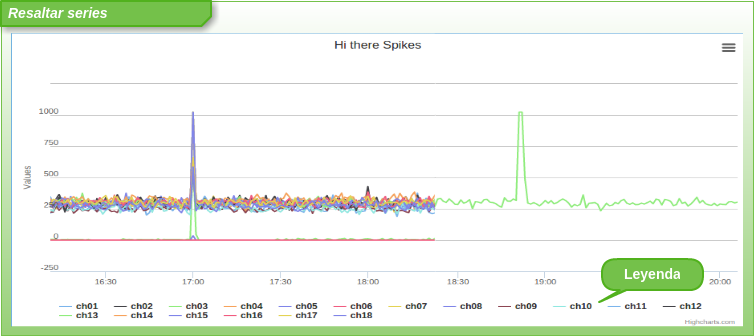
\includegraphics[keepaspectratio, width=1\textwidth]{./img/resalto.png}
				\caption{Ampliando HighStock. Resaltar series.}   
				\label{fig:resalto}
			\end{figure}
	
\section{Modelo}
	El \emph{modelo} es el encargado de manejar los datos de una aplicación. En el caso del \emph{front-end} los datos de la aplicación deben ser
	servidos por el \emph{back-end}. El \emph{modelo} es el encargado de realizar la comunicación con el \emph{back-end}. 
	\par
	Tal y como especificamos en el  capítulo anterior el protocolo para la comunicación entre los dos módulos es \emph{HTTP}. Nuestro
	\emph{front-end} es el que empieza la comunicación enviando un mensaje de petición y el \emph{back-end} responde a esa peticion con un mensaje
	de respuesta. El \emph{modelo} es el encargado de enviar los mensajes de petición y después interpretar los mensajes de respuesta.
	\par
	Para dotar el \emph{modelo} de la funcionalidad necesaria utilizamos las facilidades que ExtJs ofrece, concretamente utilizamos el singleton
	\texttt{Ext.Ajax}. Ajax\cite{AjaxWiki} es una técnica de desarrollo Web donde cliente y servidor mantienen una comunicación asíncrona en
	segundo plano. \texttt{Ext.Ajax} es un singleton de la clase \texttt{Ext.data.Connection}, clase que encapsula la lógica necesaria para
	realizar una comunicación Ajax. 
	\par
	Concretamente hacemos uso de la función \texttt{Ext.data.Connection.request}. Esta función envía una petición \emph{HTTP} a un servidor
	remoto. La función acepta únicamente un parámetro que es un objeto cuyas propiedades definen el comportamiento de la función. Las propiedades de las
	que nosotros hacemos uso están detalladas a continuación. 
	\begin{itemize}
		\item	\texttt{url}. La URL a la que enviaremos la petición. En nuestro caso \emph{back-end} y \emph{front-end} estarán albergados en
			el mismo \emph{host}. Esto nos permite no especificar el \emph{host}, la petición se hará al \emph{host} utilizado para cargar
			la aplicación. En la URL solamente hay que que especificar el servicio deseado y los parámetros que acompañan a este.
			Seguidamente presentamos un ejemplo del valor que puede tomar el campo \texttt{url}.
    				\begin{center} \texttt{url: \cc/nmdadb/channel/stats/default/default\cc}  \end{center}
		\item	\texttt{method}. El método que especifica nuestro mensaje de petición. Los mensajes \emph{HTTP} de petición pueden especificar
			un método. Si este campo es dejado vacío el método utilizado es \texttt{GET}. La mayoría de los servicios ofrecidos por el
			\emph{back-end} aceptan un método \texttt{GET}, pero el servicio \texttt{nmdbMarkNull} acepta un método \texttt{POST}.
		\item	\texttt{success}. La función a ser invocada al completar exitosamente la petición. Esta función a su vez acepta como parámetro
		  	\texttt{response}. Este parámetro contiene los datos del mensaje de respuesta.
		\item	\texttt{failure}. La función a ser invocada al completar sin éxito la petición. Esta función también acepta el parámetro
		  	\texttt{response} que podemos utilizar para identificar la causa del fallo.
		\item	\texttt{timeout}. El número de milisegundos en los que el \emph{back-end} debe responder. Si el tiempo expira la solicitud se
		  	considera como fallida. 
	\end{itemize}
	Más allá de \texttt{Ext.Ajax} el framework ofrece abstracciones de un nivel superior. La clase \texttt{Ext.data.Model} es una representación
	de un objeto utilizado por nuestra aplicación. Estos modelos son usados por la clase \texttt{Ext.data.Store}, que encapsula instancias de
	estos. Estas abstracciones son muy útiles, pero algo complejas. Al no estar acostumbrado a trabajar con estas el autor de este trabajo ha
	preferido utilizarlas lo menos posible. Por esta razón la mayoría de los datos se manejan usando el \texttt{Ext.data.Connection}, hemos
	utilizado el \texttt{Ext.data.Store} en casos muy específicos como los datos que necesitan ser mostrados en una tabla. Las tablas en ExtJs
	deben tener asociado un \texttt{Ext.data.Store} cuyos datos mostrar. A continuación podemos ver un ejemplo de como declarar un
	\texttt{Ext.data.Model} y un \texttt{Ext.data.Store} que enlazaremos a un \texttt{Ext.grid.Panel}.
	\begin{lstlisting}[style=myJs]
Ext.define('MyApp.model.MyModel',{
   extend: 'Ext.data.Model',
   fields: [	{name: 'myName1', type: 'string'},
   		{name: 'myName2', type: 'string'}]
});

Ext.define('MyApp.store.MyStore',{
   extend: 'Ext.data.Store',
   model: 'MyApp.model.MyModel',
   proxy: {
      type: 'ajax',
      url: '/nmdadb/channel/stats/default/default',
      reader: {
         type: 'json'}}
});
var myStore = Ext.create('MyApp.store.MyStore');
myStore.load();

Ext.define('MyApp.grid.MyGrid',{
   extend: 'Ext.grid.Panel',
   title: 'MyCoolGrid',
   store: myStore,
   fields: [	{text: 'Name1', dataIndex: 'myName1'},
		{text: 'Name2', dataIndex: 'myName2'}]
});
Ext.create('MyApp.grid.MyGrid', {
   renderTo: Ext.getBody()
});
	\end{lstlisting}
	\par
	Podemos ver que en la declaración del \texttt{Ext.data.Store} especificamos \texttt{proxy}. El objeto especificado es utilizado para crear una
	instancia de la clase \texttt{Ext.data.proxy.Proxy}. Esta clase es una abstracción que agrupa diferentes técnicas de comunicación como Ajax,
	JsonP, Rest y Direct.

\section{Controlador}
	El Controlador en una aplicación \emph{modelo-vista-controlador}\cite{MVCWiki} hace de intermediario entre la Vista y el Modelo. Normalmente
	este responde a los eventos producidos por el usuario. Las respuestas consisten en peticiones al Modelo para cargar datos o bien en comandos
	dirigidos a la Vista para realizar un cambio en la forma de mostrar los datos. El Controlador contiene toda la lógica de la aplicación por lo
	que podemos decir que es el módulo más interesante. El propósito de esta sección es hacer una descripción de este.
	\par
	Sencha ExtJs ofrece la clase \texttt{Ext.app.Controller}, abstracción que representa un Controlador. Esta clase contiene la funcionalidad
	mínima necesaria, está pensada para ser extendida y dotada de funcionalidad por el usuario. A continuación podemos ver un pequeño ejemplo de
	como declarar un Controlador básico en Sencha ExtJs.
	\begin{lstlisting}[style=myJs]
Ext.define('MyApp.controller.Users', {
   extend: 'Ext.app.Controller',
   onLaunch: function() {
      console.log('Podemos empezar..');}
});
	\end{lstlisting}
	\par
	La función \texttt{onLaunch()} es una función especial que es invocada después de inicializar la aplicación. La Vista y Modelo ya están
	inicializados, por lo que es un buen punto para empezar a actuar sobre estos elementos.
	\par
	Antes de empezar a discutir los Controladores que hemos implementado en este trabajo es conveniente destacar que el framework ofrece una
	facilidad similar al \texttt{Ext.ComponentQuery}, pero para los Controladores. Podemos hacer consultas para acceder a los Controladores desde
	cualquier punto del código. A continuación podemos ver como hacer uso de esta facilidad.
    		\begin{center} \texttt{MyApp.app.getController("Nombre\_del\_Controlador")}  \end{center}
	\par
	En nuestra aplicación hemos definido cinco Controladores, las subsecciones venideras son dedicadas a estos.
	\subsection{\texttt{HighStockExtend}}
		El propósito de este Controlador es inicializar las dos extensiones de HighStock que discutimos previamente en este capítulo. Este
		Controlador es invocado antes de empezar a construir los gráficos de la aplicación para que las extensiones estén listas y sean
		aplicadas a estos.
	\subsection{\texttt{Navigation}}
		Este Controlador es el encargado de inicializar el \texttt{Ext.History}, mecanismo que solventa el problema de navegación por el
		historial en aplicaciones \emph{single-page}. El problema y el mecanismo fueron descritos en secciones anteriores de este capítulo.
		\par
		El Controlador define la función \texttt{onLaunch()}, función que es invocada una vez creados la Vista y el Modelo de la aplicación.
		Empieza invocando la función \texttt{Ext.History.init()}, función esencial para inicializar este módulo. Seguidamente define la
		función encargada de manejar el evento \texttt{change}, evento que se dispara al cambiar el \emph{hash} de la URL. Esta función
		soporta tres valores diferentes como \emph{hash} que son \texttt{[Spike, SpikeRevised, ChannelStats]}. Estos tres valores representan
		los tres módulos funcionales entre los que hacemos distinción. Cambiando el \emph{hash} cambiamos el módulo funcional mostrado en
		pantalla.
		\par
		Podemos ver que el soporte de navegación por el historial es pobre en funcionalidad, por esta razón proponemos como trabajo futuro
		extender y ampliar la funcionalidad de este.
		\par
		También debemos tener en cuenta que al inicializarse la aplicación puede haber un \emph{hash} especificado. Una vez especificado el
		comportamiento ante un evento \texttt{change} procedemos a evaluar el \emph{hash} actual. Este puede no estar presente, caso en el que
		cargamos el módulo funcional \texttt{Spike}. En el caso de la presencia de un \emph{hash} actuamos conforme a este.
	\subsection{\texttt{Spike}}
		Este Controlador es directamente relacionado al módulo funcional con el mismo nombre, \texttt{Spike}. Este Controlador es algo más
		complicado que los anteriormente discutidos, este es compuesto por múltiples funciones. A continuación procedemos a explicar estas
		funciones.
		\begin{description}[style=unboxed,leftmargin=0cm]
			\item[\texttt{Launch()}] Inicializa el módulo funcional \texttt{Spike}. Es conveniente destacar que esta función no es
			  \texttt{onLauch}, esta no es invocada automáticamente al inicio de la aplicación, somos nosotros los que la invocamos. Esta
			  función inicializa el objeto \texttt{app}, objeto que debe contener todas las variables usadas en este módulo. La mayoría de
			  las demás funciones usaran este objeto para acceder a estas variables. Después de inicializar este objeto es invocada la
			  función \texttt{loadInitialData()}.
			\item[\texttt{loadInitialData()}] Esta función carga los datos necesarios para construir el módulo. Los datos son cargados
			  realizando una petición Ajax al \emph{back-end}. El servicio RPC que invocamos es \texttt{nmdbOriginalGroup}. Al cargar los
			  datos con éxito son invocadas las funciones \texttt{initCandleChart()} y \texttt{initChannelChart()}. 
			\item[\texttt{initCandleChart()}] Esta función es la encargada de crear el gráfico \emph{Candlestick} con los datos de la
			  estación. Hablaremos más a fondo sobre este gráfico en las secciones futuras donde discutiremos la herramienta desde un
			  enfoque funcional.
			\item[\texttt{initChannelChart()}] Esta función es la encargada de crear el gráfico que representa los datos de los tubos
			  contadores por separado. Igual que en el caso anterior hablaremos más sobre este gráfico en secciones futuras.
			\item[\texttt{LineOrOhcl(start, finish, N\_points)}] Anteriormente en este capítulo discutimos el problema que surge al
			  intentar representar un gran número de datos en un gráfico convencional y que el gráfico \emph{Candlestick} da solución a
			  este problema. Esta función determina si debemos utilizar un gráfico de línea o bien uno \emph{Candlestick}. La cantidad de
			  datos es definida por los parámetros \texttt{start} y \texttt{finish}, el parámetro \texttt{N\_points} representa el número
			  de pixeles que tenemos a disposición para representar los datos.
			\item[\texttt{updateMode(start, finish)}] Esta función es invocada cuando ocurre algún cambio en el gráfico \emph{Candlestick}
			  y calcula el modo en que deben ser representados los datos. Esta función hace un uso intensivo de la función
			  \texttt{LineOrOhcl()}, pero tiene en cuenta más cosas como la serie actual.
			\item[\texttt{changeSeries(series)}] Esta función cambia la serie que es presentada en el gráfico \emph{Candlestick}. El
			  parámetro \texttt{series} es un entero que puede tomar los siguientes valores \texttt{[1, 2, 3]}, donde estos representan
			  uncorrected, corrected for pressure y corrected for efficiency.
			\item[\texttt{updateSeries()}] Esta función simplemente refresca los datos de las series del gráfico \emph{CandleStick}. Es
			  invocada cada vez que ocurre algún cambio en este para refrescar los datos.
			\item[\texttt{updateCandleData(start, finish)}] Esta función carga los datos para el gráfico \emph{Candlestick} en función de
			  la petición realizada por el usuario. Para cargar los datos la función realiza una petición Ajax al \emph{back-end}. La
			  función invoca el servicio RPC \texttt{nmdbOriginalGroup} o \texttt{nmdbOriginalRaw} en función del valor devuelto por la
			  función \texttt{LineOrOhcl()}. El intervalo de datos que será solicitado es definido por los parámetros \texttt{start} y
			  \texttt{finish}. 
			\item[\texttt{updateChannelData()}] Esta función carga los datos para el gráfico que representa los datos de los tubos
			  contadores por separado. Los datos son cargado del \emph{back-end} mediante una petición Ajax que invoca el servicio RPC
			  \texttt{nmdadbRawData}.
			\item[\texttt{searchInterval(start, finish)}] Esta función permite hacer una búsqueda por intervalos temporales. El intervalo
			  es definido por los parámetros \texttt{start} y \texttt{finish}.
			\item[\texttt{getTimestamp(str)}] Esta función acepta una cadena de texto que debe seguir un formato determinado y devuelve un
			  objeto de la clase \texttt{Date}. 
			\item[\texttt{showCandle()}] Esta función muestra el gráfico \texttt{Candlestick} creado por este Controlador. Junto al
			  gráfico también se asegura de mostrar los controles vinculados a este. Si es la primera vez que intentamos mostrar este
			  gráfico el módulo entero no estará creado, esta función invoca la función \texttt{Launch()} en tal caso.
			\item[\texttt{showChannel()}] Esta función muestra el gráfico de los tubos contadores por separado. Junto al gráfico también
			  se asegura de mostrar los controles vinculados a este. Es invocada la función \texttt{updateChannelData()} para asegurar que
			  son mostrados los datos correctos.
		\end{description}
	\subsection{\texttt{SpikeRevised}}
		Este Controlador es muy similar al anteriormente descrito, \texttt{Spike}. Las diferencias como indica el nombre radican en que este
		utiliza los datos revisados, no los originales. Además de utilizar un conjunto de datos distinto este Controlador también ofrece
		funcionalidad extendida, permite marcar datos como inválidos. Los datos marcados como inválidos serán considerados nulos en el
		conjunto de datos revisados.
		\par
		A continuación procederemos a explicar las funciones que este Controlador define.
		\begin{description}[style=unboxed,leftmargin=0cm]
			\item[\texttt{Launch()}]
				Inicializa el módulo funcional \texttt{SpikeRevised}. Esta función inicializa el objeto \texttt{app} que debe contener
				todas las variables asociadas a este módulo. La estructura de este objeto es idéntica al objeto creado en la función
				\texttt{Launch()} del Controlador \texttt{Spike} a excepción de una serie de atributos extra. 
				\par
				Seguidamente son importadas todas las funciones que podemos reutilizar del Controlador \texttt{Spike}, de esta forma
				se evita duplicar código idéntico. Las funciones importadas son listadas a continuación.
					\begin{center} \texttt{	initCandleChart, initChannelChart, changeSeries, searchInterval, updateChannelData,
					  			LineOrOhcl, updateMode, updateSeries, getTimestamp}
					\end{center}
				Finalmente es invocada la función \texttt{loadInitialData()}.
		    	\item[\texttt{loadInitialData()}]
				Esta función es muy parecida a la función con el mismo nombre del Controlador \texttt{Spike}. La función carga los
				datos necesarios para construir el módulo. La diferencia radica en el servicio RCP utilizado. Esta función utiliza el
				servicio \texttt{nmdbRevisedGroup}, tal y como explicamos este módulo utiliza los datos revisados.
				\par
				Al cargar los datos con éxito son invocadas las funciones \texttt{initCandleChart} y \texttt{initChannelChart} que
				crean los dos gráficos, estas son función importadas del Controlador \texttt{Spike}. Finalmente es invocada la función
				\texttt{extendChandleChart} que será explicada a continuación.
			\item[\texttt{extendCandleChart()}]
				Volvemos a recordar que este módulo es muy similar al \texttt{Spike}, pero ofrece alguna funcionalidad extra. Esta
				función es la encargada de extender la funcionalidad del gráfico \emph{Candlestick}. La función define el
				comportamiento de las series del gráfico ante el evento \texttt{click}. Este comportamiento consiste en marcar el dato
				con un flag y añadirlo a una tabla. Posteriormente los datos en la tabla podrán ser clasificados como inválidos. 
			\item[\texttt{updateCandleData(start, finish)}]
				Esta función es muy parecida a la función con el mismo nombre del Controlador \texttt{Spike}. La función carga los
				datos para el gráfico Candlestick en función de la petición realizada por el usuario. La diferencia radica en los
				servicios RPC utilizados. Esta función utiliza lo servicios \texttt{nmdbRevisedGroup} o \texttt{nmdbRevisedRaw} en
				función del valor devuelto por la función \texttt{LineOrOhcl()}.El intervalo de datos que es solicitado es definido
				por los parámetros \texttt{start} y \texttt{finish}.
			\item[\texttt{removeFromGrid(rowIndex)}]
				Los datos marcados son guardados en una tabla. Esta función permite eliminar un dato de esta tabla. El parámetro que
				esta función acepta especifica el dato que será eliminado de la tabla. 
			\item[\texttt{submitGrid()}]
				Esta función permite clasificar como inválidos los datos en la tabla. La función invoca el servicio
				\texttt{nmdbMarkNull} del \emph{back-end} a fin de cumplir con su propósito. Una vez anulados correctamente los datos,
				la tabla es vaciada y el gráfico refrescado a fin de mostrar los cambios.
			\item[\texttt{showHideGrid()}]
				Esta función permite mostrar u ocultar la tabla que contiene los datos marcados, de esta manera los datos pueden ser
				inspeccionados.
			\item[\texttt{clearGrid()}]
				Esta función permite vaciar la tabla que contiene los datos marcados, de esta manera estos son descartados y no es
				tomada ninguna acción.
			\item[\texttt{showCandle()}]
				Esta función es muy parecida a la función con el mismo nombre del Controlador \texttt{Spike}. La función muestra el
				gráfico \emph{Candlestick} y todos los controles vinculados a este. La función \texttt{Launch()} es invocada en el
				caso de que el módulo no esté creado.
			\item[\texttt{showChannel()}]
				Esta función es muy parecida a la función con el mismo nombre del Controlador \texttt{Spike}. La función muestra el
				gráfico de los tubos contadores por separado. Junto al gráfico también se asegura de mostrar los controles vinculados
				a este. Es invocada la función \texttt{updateChannelData()} para asegurar que son mostrados los datos correctos.
		\end{description}
	\subsection{\texttt{ChannelStats}}
		Este Controlador es directamente relacionado con el módulo funcional con el mismo nombre, \texttt{ChannelStats}. Este controlador es
		compuesto por varias funciones que discutiremos a continuación.
		\begin{description}[style=unboxed,leftmargin=0cm]
			\item[\texttt{Launch()}]
				Inicializa el módulo funcional \texttt{ChannelStats}. Esta función inicializa el objeto \texttt{app}, objeto que debe
				contener todas las variable usadas en este módulo. Después de iniciar este objeto es invocada la función
				\texttt{loadInitialData()}.
			\item[\texttt{loadInitialData()}]
				Esta función carga los datos necesarios para construir el módulo. Los datos son cargados realizando una petición Ajax
				al \emph{back-end}. Son invocados dos servicios RPC, \texttt{nmdadbChannelStats} y \texttt{nmdadbChannelHistogram}. El
				primero devuelve una serie de estadísticas descriptivas de los canales, estos datos son representados en un gráfico y
				también listados en una tabla. El segundo carga los datos necesarios para construir un histograma de la distribución
				de cuentas para los 18 canales.
				\par
				Al cargar los datos con éxito son invocadas las funciones \texttt{initStatsChart()} y \texttt{initHistogramChart()}
				que  crean los dos gráficos, el gráfico con las estadísticas y el histograma. Los datos de la tabla son actualizados
				automáticamente, por lo que no tenemos que tomar ninguna acción.
			\item[\texttt{initStatsChart()}]
				Esta función es la encargada de crear el gráfico a partir de los datos devueltos por el serviocio RPC
				\texttt{nmdadbChannelStats}. 
			\item[\texttt{initChannelHistogram()}]
				Esta función es la encargada de crear el histograma que representa la distribución de cuentas para los 18 canales de
				la estación.
			\item[\texttt{searchInterval()}]
				La función que carga los datos iniciales carga los datos del último mes, esta función permite solicitar otro intervalo
				temporal. Este intervalo es definido por los dos parámetros que esta función acepta, \texttt{start} y \texttt{finish}.
				La función invoca los servicios RPC \texttt{nmdadbChannelStats} y \texttt{nmdadbChannelHistogram} para solicitar los
				datos al \emph{back-end}.
			\item[\texttt{showModule()}]
				Esta función muestra en pantalla este módulo funcional. En el caso de que este módulo no esté creado es invocada la
				función \texttt{Launch()}.
		\end{description}
	\subsection{Visión general}
		En la figura \ref{fig:controllers} podemos ver un diagrama que representa los Controladores que acabamos de explicar. En color azul
		podemos ver las funciones, gris en caso de que sean funciones importadas desde otro Controlador. Las flecha azules que unen las
		funciones muestras como estas se invocan unas a otras. Algunas funciones son invocadas al producirse un cierto evento, estos pueden
		verse en verde dentro de las funciones. Todos los eventos son producidos por los elementos que forman la Vista de la aplicación, a
		excepción del evento \texttt{Ext.History.change} que es disparado al realizar un cambio en la pila de historial de navegación.
		\begin{figure}[h]
			\centering
			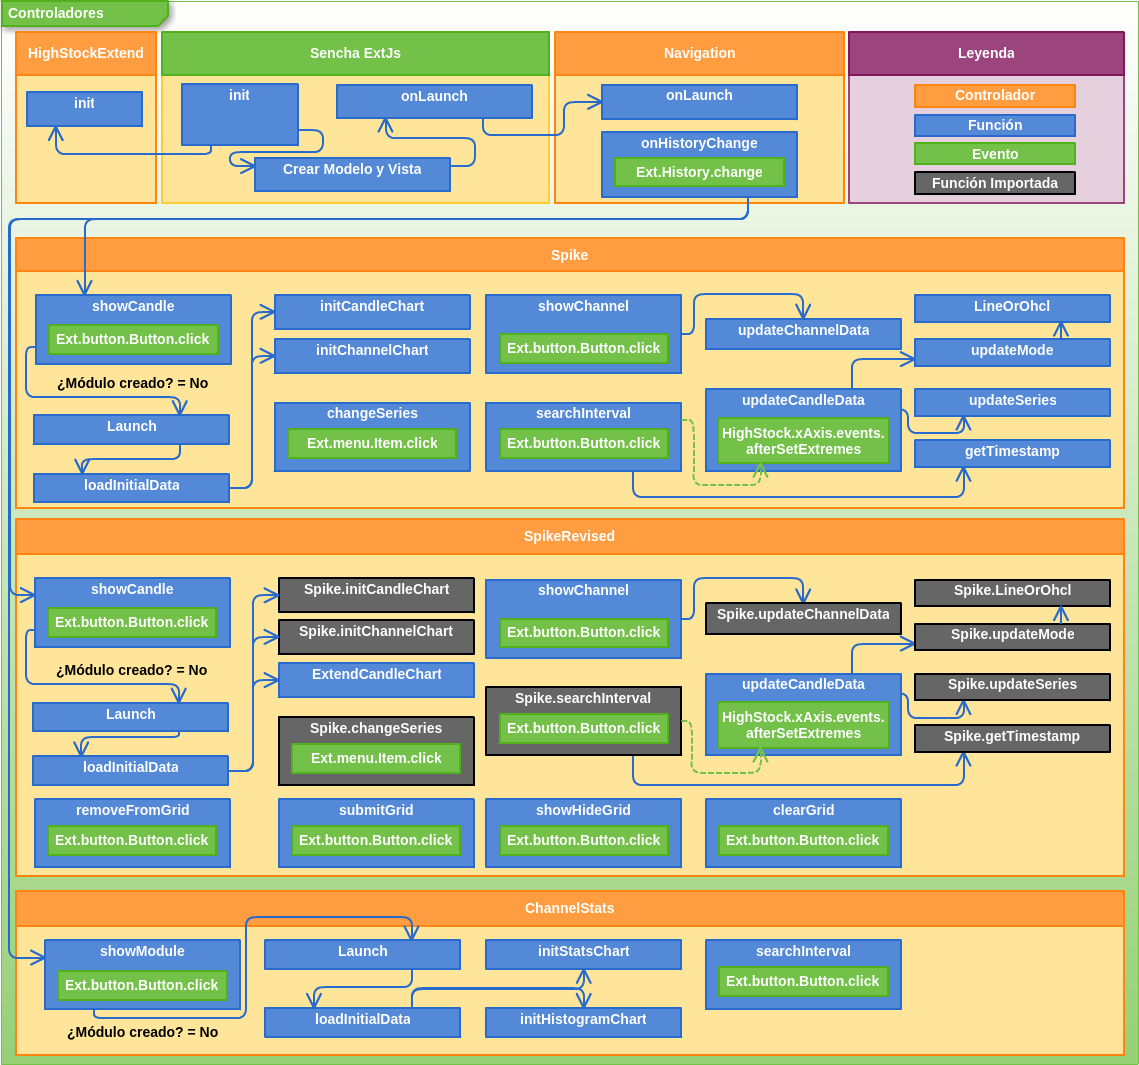
\includegraphics[keepaspectratio, width=1\textwidth]{./img/controllers.png}
			\caption{Visión general de los Controladores.}   
			\label{fig:controllers}
		\end{figure}
\section{Vista}
	El componente de Vista en una aplicación \emph{modelo-vista-controlados}\cite{MVCWiki} es el responsable de presentar la información de la
	implicación junto a todos los componentes que componen la interfaz de usuario.  El propósito de esta sección es describir los aspectos básicos
	de este componente.
	\begin{figure}[h]
		\centering
		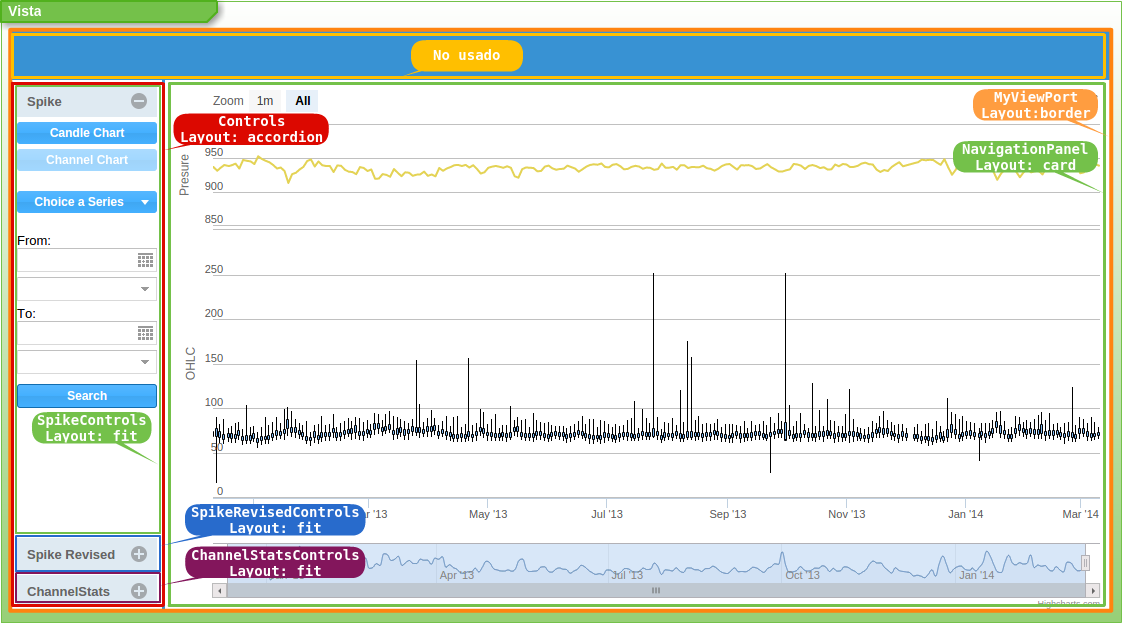
\includegraphics[keepaspectratio, width=1\textwidth]{./img/vista.png}
		\caption{\emph{Front-end}. Vista.}   
		\label{fig:vista}
	\end{figure}
	\par
	La Vista en una aplicación ExtJs es compuesta por una jerarquía de \emph{componentes}. En nuestro caso en lo más alto de esta jerarquía
	tenemos un \texttt{ViewPort} al que hemos asignado el nombre \texttt{MyViewPort}. Este es un \emph{componente} que se ajusta al área de
	aplicación disponible. El layout que determina como se posicionan los hijos de este \emph{componente} es \texttt{border}. Los
	\emph{componentes} hijos deben especificar el atributo \texttt{region} que determina su posicionamiento.
	\par
	El primer hijo con \texttt{region:north} es un \texttt{Ext.container.Container}, clase que especifica un \emph{contenedor} base. Actualmente este
	\emph{contenedor} no tiene ninguna funcionalidad, en un futuro se plantea visualizar mensajes de alerta.
	\par
	El segundo hijo del \texttt{MyViewPort} con \texttt{region:west} es también una instancia de la clase \texttt{Ext.container.Container}. El
	\texttt{itemId} que define es \texttt{Controls}. Este \emph{contenedor} tiene tres hijos que son instancias de la misma clase. Estos tres
	hijos contienen los controles vinculados a los tres módulos funcionales. Los \texttt{itemId} que estos tres hijos especifican son:
    		\begin{center} \texttt{[SpikeControls, SpikeRevisedControls, ChannelStatsControls]}  \end{center}
	\texttt{Controls} usa el layout \texttt{accordion}, donde solamente uno de los hijos puede estar expandido y los demás están
	colapsados, de esta manera no pueden ser visibles lo controles de dos módulos funcionales a la vez. Cada vez que son expandidos los
	controles de un módulo funcional el evento \texttt{Ext.panel.Panel.beforeexpand} es disparado. El handler asociado a este evento
	invoca la función apropiada de los Controladores para mostrar el módulo funcional al que pertenecen los controles que acaban de ser
	expandidos.
	\par
	La tercer hijo del \texttt{MyViewPort} con \texttt{region:center} es también una instancia de la clase \texttt{Ext.container.Container}. El
	\texttt{ítemId} que identifica a este componente es \texttt{NavigationPanel}. El layout utilizado es \texttt{card} donde los hijos se solapan
	unos a otros y tan sólo uno puede ser visible a la vez. Los \emph{componentes} hijos contienen todos los gráficos y tablas que nuestra
	aplicación ofrece, estos son mostrados en función del estado de los controles.
	\par
	En la figura \ref{fig:vista} podemos ver como se organizan los componentes de la Vista que acabamos de explicar.
\section{Descripción funcional}
	El propósito de esta sección es hacer una descripción funcional de la herramienta. Diferenciamos entre tres módulos funcionales que son
	\texttt{Spike}, \texttt{SpikeRevised} y \texttt{ChannelStats}.
	\subsection{\texttt{Spike}}
		El propósito de este módulo es ofrecer un gráfico interactivo que permite localizar los \emph{spikes} de forma fácil. Recordamos
		que estos son datos anormalmente grandes o pequeños. La figura \ref{fig:spikeRevised} presenta el módulo funcional
		\texttt{SpikeRevised}, dado que los dos módulos son muy similares podemos fijarnos en esta figura.
		\par
		Inicialmente el módulo tiene que representar todos los datos de la estación, razón por la que es utilizado el gráfico
		\emph{Candlestick}. En este gráfico los valores máximo y mínimo para cada grupo son fáciles de distinguir. Eventualmente cuando es
		solicitado un intervalo temporal para el que no es necesario agrupar los datos, el gráfico automáticamente cambia a un gráfico de
		línea. Por contrario si se vuelve a solicitar un intervalo que requiere agrupar los datos, el gráfico cambia a \emph{Candlestick}.
		\par
		Para solicitar un intervalo diferente de datos tenemos varias facilidades. La primera es el zoom interactivo que podemos realizar
		haciendo \emph{click} y arrastrando sobre un intervalo del gráfico. Dependiendo de la dirección de arrastre este será un zoom In u
		Out. La segunda alternativa es utilizar los campos de entrada disponibles en los controles para realizar una búsqueda por intervalo.
		En estos campos podemos especificar el inicio y fin del intervalo y la búsqueda será realizada al accionar el botón de búsqueda. La
		tercera opción es utilizar el navegador que podemos encontrar en la parte inferior del gráfico. Finalmente podemos utilizar los
		botones en la parte superior izquierda, \texttt{1m} y \texttt{All} del gráfico que permiten fijar un intervalo de un mes o volver
		a mostrar todos los datos.
		\par
		Inicialmente son mostrados los datos sin corregir, utilizando el botón \texttt{Choise a Series} podemos mostrar los datos corregidos
		por presión o los corregidos por eficiencia. En la parte superior del gráfico son representados los valores de la presión atmosférica,
		estos permiten correlacionar los datos respecto a esta magnitud.
		\par
		Cuando no es necesario agrupar los datos el botón \texttt{Channel Chart} es habilitado. Este botón muestra un gráfico secundario con
		los valores de los tubos contadores por separado. El intervalo de datos es marcado por el intervalo del gráfico principal. Este
		gráfico permite observar el comportamiento de los diferentes tubos. El botón \texttt{Candle Chart} permite volver al gŕafico
		principal.
	\subsection{\texttt{SpikeRevised}}
		Este módulo funcional incorpora toda la funcionalidad del módulo anterior, la diferencia radica en que este utiliza un conjunto de
		datos diferente y además ofrece alguna funcionalidad extra. \texttt{Spike} utiliza los datos originales, mientras que este módulo
		utiliza los datos revisados. La funcionalidad extra que este módulo ofrece permite añadir datos al conjunto de datos revisados.
		\par
		Para satisfacer dicha funcionalidad este módulo ofrece una tabla. Esta tabla es mostrada en una ventana separa que puede ser mostrada
		u ocultada utilizando el botón \texttt{Selected Points}. Los datos de esta tabla pueden ser enviados al conjunto de datos revisados
		utilizando el botón \texttt{Submit} que está presente en la misma ventana. Los datos añadidos a este conjunto serán considerados como
		nulos en el futuro. Este botón además de enviar los datos actualiza el gráfico para reflejar los cambios que acaban de producir se.
		\par
		Cuando los datos son representados en modo línea podemos hacer \emph{click} sobre un dato para añadir este a la tabla anteriormente
		descrita. En el gráfico es añadido un \emph{flag}, la letra que aparece en dicho \emph{flag} se corresponde con el campo
		\texttt{Label} de la tabla.
		\begin{figure}[h]
			\centering
			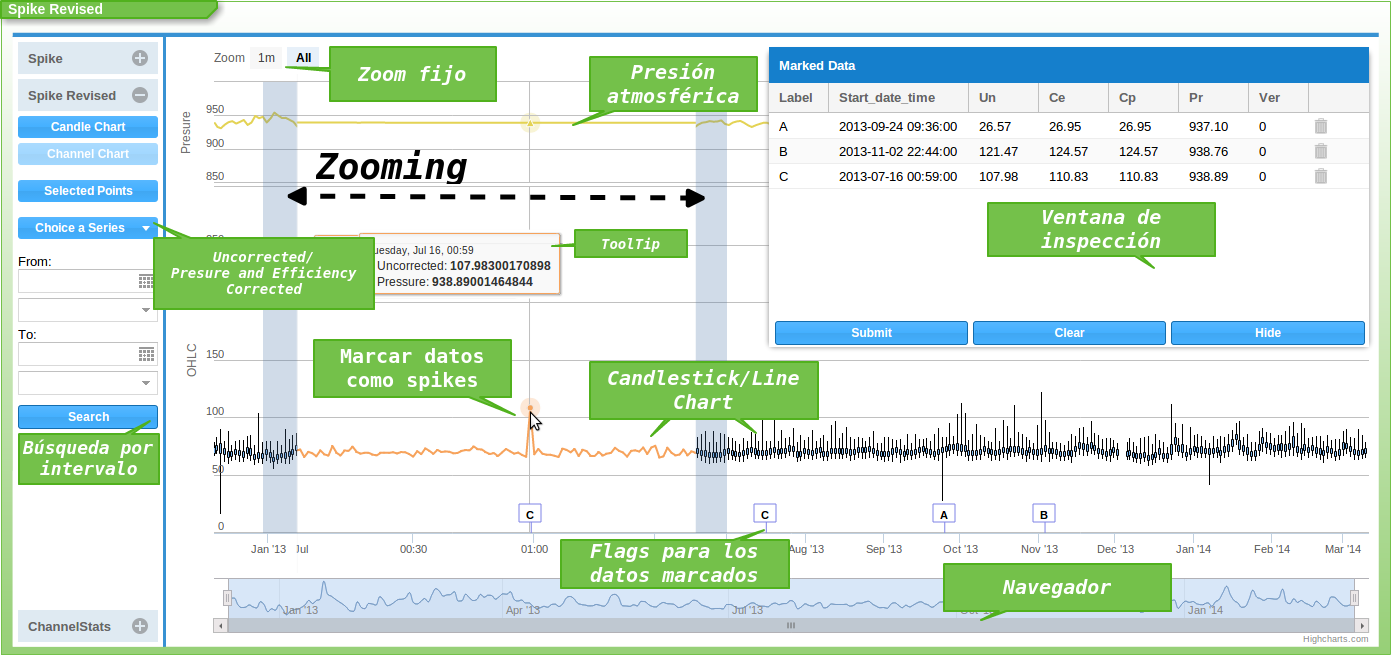
\includegraphics[keepaspectratio, width=1\textwidth]{./img/spikeRevised.png}
			\caption{Descripción funcional. SpikeRevised}   
			\label{fig:spikeRevised}
		\end{figure}
	\subsection{\texttt{ChannelStats}}
		El propósito de este módulo funcional es ofrecer información de los diferentes canales por separado, de esta manera somos capaces de
		identificar mal funcionamientos en canales aislados. El módulo ofrece una tabla en la que podemos inspeccionar la media, desviación
		típica, máximo, mínimo y último valor para cada canal. Estos datos también son representados en un gráfico \emph{Candlestick}.
		\par
		Junto a estos datos el módulo ofrece un histograma con la distribución de cuentas para los diferentes canales. Dicho histograma puede
		ser visto en una pestaña separada.
		\par
		Inicialmente los datos y el histograma son calculados para el último mes. En los controles podemos encontrar los campos de entrada que
		permiten solicitar un intervalo de tiempo determinado. La búsqueda por intervalo está limitada a un mes dado a que las consultas
		necesarias para obtener estos datos no son muy efficientes, estas agrupan los datos por campos que no están indexados. Más sobre este
		problema podemos encontrar en el capítulo dedicado al \emph{back-end}.
